\documentclass[a4paper,12pt,twocolumn,landscape]{article}

\usepackage{superpack2015}

\usepackage{vecteurs1-activite4-zellige-numero}	% Activité pavage Zellige

\usepackage[heightrounded]{geometry}	% heightrounded permet d'afficher les footers correctement
\geometry{hmargin=0.5cm,vmargin=1.5cm}

\setlength{\columnseprule}{0.5pt}		% Ligne séparatrice milieu document
\setlength{\columnsep}{50pt}			% Espace de chaque côté de la ligne
\setlength{\headsep}{15pt}
\addtolength{\textheight}{40pt}
%\setlength{\textwidth}{770pt}
%\setlength{\hoffset}{20pt}

\classichf
	% Nom du style
	{activite}
	% Hauteur sous header
	% 14.5pt si une ligne (1 \baselineskip)
	% 29.0pt si deux lignes (2 \baselineskip)
	{14.5pt}
	% Head
	{}
	{\textbf{Activités : Les vecteurs}}
	{}
	% Foot
	{}
	{}
	{}

\classichf
	% Nom du style
	{activite-reponses}
	% Hauteur sous header
	% 14.5pt si une ligne (1 \baselineskip)
	% 29.0pt si deux lignes (2 \baselineskip)
	{14.5pt}
	% Head
	{}
	{\textbf{Activités : Les vecteurs (réponses)}}
	{}
	% Foot
	{}
	{}
	{}

\renewcommand{\vect}[9]{
	\coordinate(#1) at (#3,#4);
	\coordinate(#2) at (#5,#6);
	\draw (#1) -- (#2) node [fill=white,midway,above,sloped] {
	%$\textcolor{#9}{\overrightarrow{#1#2}}$
	};
	\draw (#1) node [fill=white,#7] {#1};
	\draw (#2) node [fill=white,#8] {#2};
	\draw [->,>=stealth,line width=1.5pt] (#1) -- (#2);
}


\begin{document}

\thispagestyle{activite}
\begin{minipage}{0.45\textwidth}

\paragraph{Activité~1} Retrouvez les vecteurs égaux.

\begin{center}
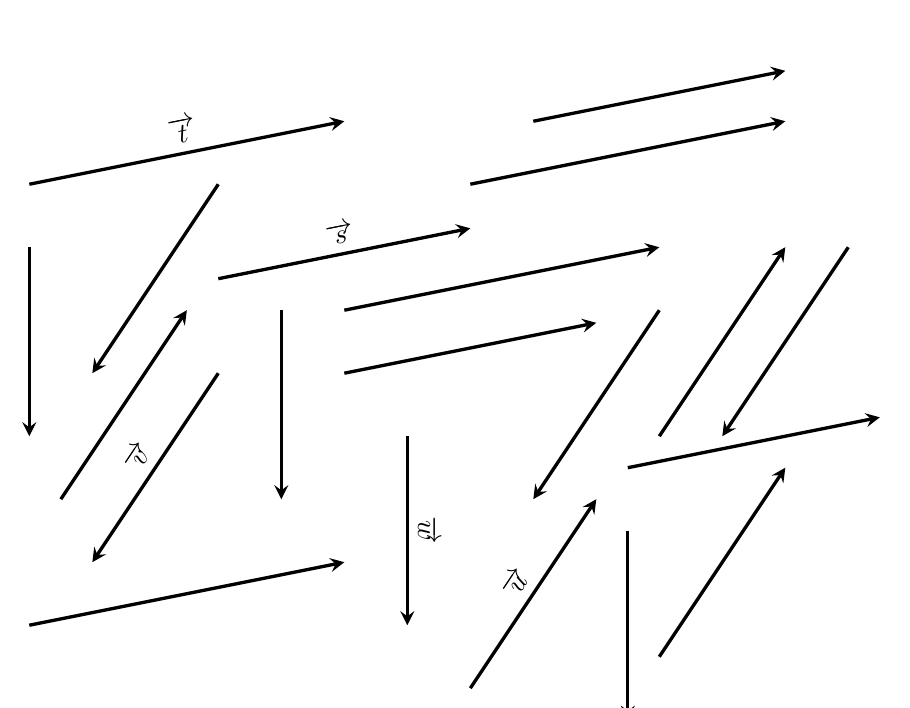
\begin{tikzpicture}[scale=0.8,every node/.style={scale=1}]
	\tikzstyle{vect}=[->,>=stealth,very thick]
	\tikzstyle{vectred}=[vect]
	\tikzstyle{vectblue}=[vect]
	\tikzstyle{vectgreen}=[vect]
	\tikzstyle{vectgray}=[vect]
	\tikzstyle{vectcyan}=[vect]
	

\coordinate (A) at (2,2);
\coordinate (B) at (5,6);
\coordinate (C) at (-4.5,5);
\coordinate (D) at (5,2.5);
\coordinate (u) at (2,3);
\draw[vectred] (A) -- ++ (u) node[midway, sloped, above]{$\overrightarrow{u}$};
\foreach \point in {B, C, D}
	\draw[vectred] (\point) -- ++ (u);

\coordinate (E) at (-2,7);
\coordinate (F) at (-2,10);
\coordinate (G) at (8,9);
\coordinate (H) at (5,8);
\coordinate (v) at (-2,-3);
\draw[vectblue] (E) -- ++ (v) node[midway, sloped, above]{$\overrightarrow{v}$};
\foreach \point in {F, G, H}
	\draw[vectblue] (\point) -- ++ (v);

\coordinate (I) at (1,6);
\coordinate (J) at (-1,8);
\coordinate (K) at (4.5,4.5);
\coordinate (L) at (-5,9);
\coordinate (w) at (0,-3);
\draw[vectgreen] (I) -- ++ (w) node[midway, sloped, above]{$\overrightarrow{w}$};
\foreach \point in {J, K, L}
	\draw[vectgreen] (\point) -- ++ (w);

\coordinate (M) at (-5,10);
\coordinate (N) at (-5,3);
\coordinate (O) at (0,8);
\coordinate (P) at (2,10);
\coordinate (t) at (5,1);
\draw[vectgray] (M) -- ++ (t) node[midway, sloped, above]{$\overrightarrow{t}$};
\foreach \point in {N, O, P}
	\draw[vectgray] (\point) -- ++ (t);

\coordinate (Q) at (-2,8.5);
\coordinate (R) at (4.5,5.5);
\coordinate (S) at (0,7);
\coordinate (T) at (3,11);
\coordinate (s) at (4,0.8);
\draw[vectcyan] (Q) -- ++ (s) node[midway, sloped, above]{$\overrightarrow{s}$};
\foreach \point in {R, S, T}
	\draw[vectcyan] (\point) -- ++ (s);
\end{tikzpicture}
\end{center}

\paragraph{Activité~3} Complétez les égalités suivantes~:\\
%\begin{center}
\begin{minipage}{0.5\textwidth}
\begin{tikzpicture}[scale=0.75,every node/.style={scale=1}]
	\tikzstyle{vect}=[->,>=stealth,ultra thick]
	
	\clip (-1,-1) rectangle (5,5);
	\placerpoint{A}{1}{2}{above left}
	\placerpoint{B}{2}{3}{above left}
	\placerpoint{C}{3}{2}{above right}
	\placerpoint{D}{2}{1}{below left}
	\draw (A) -- (B) -- (C) -- (D) -- cycle;
	\draw[vect] (A) -- (B);
	\draw[vect] (B) -- (C);
	\draw[vect] (A) -- (D);
	\draw[vect] (D) -- (C);
	\draw (0,0) grid (4,4);
\end{tikzpicture}
\end{minipage}
\begin{minipage}{0.5\textwidth}
\vectaffiche{AB} + \vectaffiche{BC} = \\
\vectaffiche{AD} + \vectaffiche{DC} = \\[1em]
\vectaffiche{AD} + \vectaffiche{CB} + \vectaffiche{AB} = \\
\end{minipage}

\begin{minipage}{0.5\textwidth}
\begin{tikzpicture}[scale=0.75,every node/.style={scale=1}]
	\tikzstyle{vect}=[->,>=stealth,ultra thick]
	
	\placerpoint{E}{0}{2}{above left}
	\placerpoint{F}{2}{4}{above left}
	\placerpoint{G}{4}{2}{above right}
	\placerpoint{H}{2}{0}{below left}
	\draw (E) -- (F) -- (G) -- (H) -- cycle;
	\draw[vect] (E) -- (F);
	\draw[vect] (F) -- (G);
	\draw[vect] (E) -- (H);
	\draw[vect] (H) -- (G);
	\draw (-1,-1) grid (5,5);
\end{tikzpicture}
\end{minipage}
\begin{minipage}{0.5\textwidth}
\vectaffiche{EF} + \vectaffiche{FH} + \vectaffiche{HG} = \\
\vectaffiche{EH} + \vectaffiche{HF} + \vectaffiche{FG} = \\[1em]
\vectaffiche{EG} + \vectaffiche{FE} = \\
\vectaffiche{EH} + \vectaffiche{EF} = \\[1em]
\vectaffiche{FH} + \vectaffiche{EF} = \\
\vectaffiche{GE} + \vectaffiche{FG} + \vectaffiche{EF} = \\[1em]
\end{minipage}



\vspace{-4em}


\end{minipage}
\newpage

\begin{minipage}{0.45\textwidth}
\thispagestyle{activite}

\paragraph{Activité~2} ~\\

%\section{Définitions}

%\vfill
\begin{center}
\begin{tikzpicture}[scale=0.8,every node/.style={scale=0.7}]
	\tikzstyle{vect}=[->,>=stealth,very thick]
%	\clip (0.1,0.1) rectangle (14.9,9.9);
	\grille{0}{0}{15}{10}{help lines};
	\vect{A}{B}{2}{4}{3}{8}{left}{right}{red};
%	\vect{C}{D}{4}{6}{4}{2}{above}{below}{red};
	\vect{C}{D}{11}{8}{14}{9}{left}{right}{red};
	\vect{E}{F}{14}{1}{12}{4}{right}{left}{red};
	\placerpoint{M}{7}{3}{left}
%	\draw[vect,red,line width=1.5pt] (M) -- ++ (3,1);
%	\draw[vect,red,line width=1.5pt] (M) ++ (3,1) -- ++ (-2,3);
%	\draw[vect,<-,red,line width=1.5pt] (M) ++ (3,1) ++ (-2,3) -- (M);
\end{tikzpicture}
\end{center}

\begin{enumerate}
	\item Sur la figure ci-dessus, placer N image de M par la translation qui envoie C en D.
	\item Ensuite, placer O image de N par la translation qui envoie E en F.
	\item Que peut on dire de $\overrightarrow{AB}$ et de $\overrightarrow{MO}$~?
	\item Quelle est la nature du quadrilatère ABOM~?
\end{enumerate}
%\end{center}

\end{minipage}

\newpage
\thispagestyle{activite}

\paragraph{Activité~4} Zellige\\

Cette activité consiste à étudier l'enchaînement de deux translations sur un damier de carreaux Zellige, un carrelage décoratif originaire de l'Antiquité Méditerranéenne et du Moyen Orient.\\

\begin{tikzpicture}[scale=0.45,line cap=round,line join=round,>=triangle 45,x=1.0cm,y=1.0cm]
\pgfmathsetmacro{\nbSurY}{7}
\pgfmathsetmacro{\nbSurX}{6}
%
\pgfmathsetmacro{\YY}{(\nbSurY - 1) * 4}
\pgfmathsetmacro{\XX}{(\nbSurX - 1) * 4}
\pgfmathsetmacro{\grilleYY}{(\nbSurY + 1) * 4 - 1}
\pgfmathsetmacro{\grilleXX}{(\nbSurX + 1) * 4}


\grille{0}{0}{\grilleXX}{\grilleYY}{help lines}
\foreach \y in {0, 4, 8, ..., \YY}{
%\pgfmathsetmacro{\Y}{\y}
	\foreach \x in {0, 4, 8, ..., \XX}{
%	\pgfmathsetmacro{\X}{\x}
	\pgfmathsetmacro{\numero}{(0.25*(\y*6+\x)+1)}
		\begin{scope}[shift={(\x cm, \y cm)}]
		\placerpointsansnom{A}{4}{6}{above left};
		\placerpointsansnom{B}{5}{5}{above right};
		\placerpointsansnom{C}{7}{5}{above right};
		\placerpointsansnom{D}{5}{3}{above left};
		\placerpointsansnom{E}{6}{1}{below right};
		\placerpointsansnom{F}{5}{1}{below left};
		\placerpointsansnom{G}{4}{2}{above left};
		\placerpointsansnom{H}{3}{1}{below right};
		\placerpointsansnom{I}{2}{1}{below left};
		\placerpointsansnom{J}{1}{3}{above left};
		\placerpointsansnom{K}{3.5}{3.5}{above left};
			\fill[lightgray] (K) circle(1);
			\draw (K) node {\pgfmathprintnumber{\numero}};
			\draw[very thick] (A)--(B)--(C)--(D)--(E)--(F)--(G)--(H)--(I)--(J)--cycle;
		\end{scope}
	}
}
\vectAuColor{r}{18}{1}{4}{4}{4pt}{-0.1}{below}{red};
\vectAuColor{s}{19}{29}{8}{0}{4pt}{1}{right}{red};
\vectAuColor{t}{14}{5}{0}{-4}{4pt}{1.1}{below}{red};
\vectAuColor{u}{1}{15}{12}{-8}{4pt}{0}{left}{red};
\vectAuColor{v}{10}{5}{-4}{-4}{4pt}{1.1}{below}{red};
\vectAuColor{w}{9}{25}{12}{-4}{4pt}{0.4}{above}{red};
\end{tikzpicture}

\newpage

\vspace*{4em}

\begin{enumerate}
	\item Enchaînement 1
	\vspace{-2em}
		\begin{enumerate}
			\item Quelle est l'image du carreau \zellige{26} par la translation de vecteur \vectaffiche{u}~?
			\item Quelle est l'image de cette image par la translation de vecteur~\vectaffiche{v}~?
			\item Émettre une conjecture sur la nature de la transformation correspondant à l'enchaînement de ces deux translations.
		\end{enumerate}
\end{enumerate}
	\fbox{On notera \vectaffiche{u} + \vectaffiche{v} les caractéristiques de cette nouvelle transformation}\\[2em]
\begin{enumerate}
	\setcounter{enumi}{1}
	\item Enchaînement 2
	\vspace{-2em}
		\begin{enumerate}
			\item Quelle est l'image du carreau \zellige{38} par la translation de vecteur \vectaffiche{s}~?
			\item Quelle est l'image de cette image par la translation de vecteur~\vectaffiche{t}~?
			\item Émettre une conjecture sur \vectaffiche{s} + \vectaffiche{t}.
		\end{enumerate}~\\[1em]
	\item Enchaînement 3
	\vspace{-2em}
		\begin{enumerate}
			\item Quelle est l'image du carreau \zellige{22} par la translation de vecteur \vectaffiche{v}~?
			\item Quelle est l'image de cette image par la translation de vecteur~\vectaffiche{r}~?
			\item Émettre une conjecture sur \vectaffiche{v} + \vectaffiche{r}.
		\end{enumerate}
\end{enumerate}

\newpage

\thispagestyle{activite-reponses}
\begin{minipage}{0.45\textwidth}

\paragraph{Activité~1} Retrouvez les vecteurs égaux.

\begin{center}
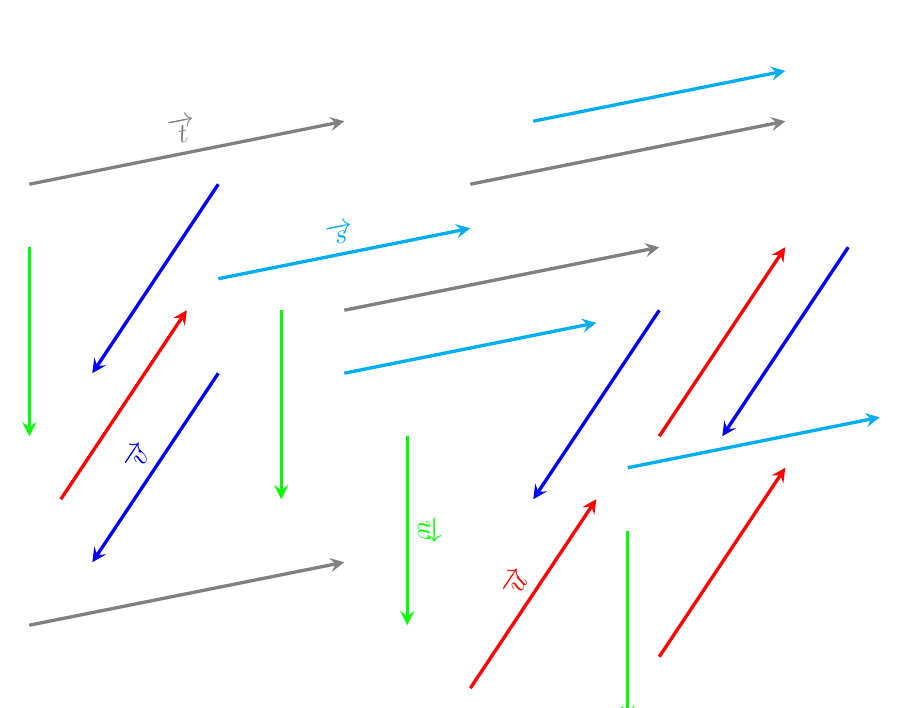
\begin{tikzpicture}[scale=0.8,every node/.style={scale=1}]
	\tikzstyle{vect}=[->,>=stealth,very thick]
	\tikzstyle{vectred}=[vect,red]
	\tikzstyle{vectblue}=[vect,blue]
	\tikzstyle{vectgreen}=[vect,green]
	\tikzstyle{vectgray}=[vect,gray]
	\tikzstyle{vectcyan}=[vect,cyan]
	

\coordinate (A) at (2,2);
\coordinate (B) at (5,6);
\coordinate (C) at (-4.5,5);
\coordinate (D) at (5,2.5);
\coordinate (u) at (2,3);
\draw[vectred] (A) -- ++ (u) node[midway, sloped, above]{$\overrightarrow{u}$};
\foreach \point in {B, C, D}
	\draw[vectred] (\point) -- ++ (u);

\coordinate (E) at (-2,7);
\coordinate (F) at (-2,10);
\coordinate (G) at (8,9);
\coordinate (H) at (5,8);
\coordinate (v) at (-2,-3);
\draw[vectblue] (E) -- ++ (v) node[midway, sloped, above]{$\overrightarrow{v}$};
\foreach \point in {F, G, H}
	\draw[vectblue] (\point) -- ++ (v);

\coordinate (I) at (1,6);
\coordinate (J) at (-1,8);
\coordinate (K) at (4.5,4.5);
\coordinate (L) at (-5,9);
\coordinate (w) at (0,-3);
\draw[vectgreen] (I) -- ++ (w) node[midway, sloped, above]{$\overrightarrow{w}$};
\foreach \point in {J, K, L}
	\draw[vectgreen] (\point) -- ++ (w);

\coordinate (M) at (-5,10);
\coordinate (N) at (-5,3);
\coordinate (O) at (0,8);
\coordinate (P) at (2,10);
\coordinate (t) at (5,1);
\draw[vectgray] (M) -- ++ (t) node[midway, sloped, above]{$\overrightarrow{t}$};
\foreach \point in {N, O, P}
	\draw[vectgray] (\point) -- ++ (t);

\coordinate (Q) at (-2,8.5);
\coordinate (R) at (4.5,5.5);
\coordinate (S) at (0,7);
\coordinate (T) at (3,11);
\coordinate (s) at (4,0.8);
\draw[vectcyan] (Q) -- ++ (s) node[midway, sloped, above]{$\overrightarrow{s}$};
\foreach \point in {R, S, T}
	\draw[vectcyan] (\point) -- ++ (s);
\end{tikzpicture}
\end{center}

\paragraph{Activité~3} Complétez les égalités suivantes~:\\
%\begin{center}
\begin{minipage}{0.5\textwidth}
\begin{tikzpicture}[scale=0.75,every node/.style={scale=1}]
	\tikzstyle{vect}=[->,>=stealth,ultra thick]
	
	\clip (-1,-1) rectangle (5,5);
	\placerpoint{A}{1}{2}{above left}
	\placerpoint{B}{2}{3}{above left}
	\placerpoint{C}{3}{2}{above right}
	\placerpoint{D}{2}{1}{below left}
	\draw (A) -- (B) -- (C) -- (D) -- cycle;
	\draw[vect] (A) -- (B);
	\draw[vect] (B) -- (C);
	\draw[vect] (A) -- (D);
	\draw[vect] (D) -- (C);
	\draw (0,0) grid (4,4);
\end{tikzpicture}
\end{minipage}
\begin{minipage}{0.5\textwidth}
\vectaffiche{AB} + \vectaffiche{BC} = \reponseEX{\vectaffiche{AC}} \\
\vectaffiche{AD} + \vectaffiche{DC} = \reponseEX{\vectaffiche{AC}}\\[1em]
\vectaffiche{AD} + \vectaffiche{CB} + \vectaffiche{AB} = \reponseEX{\vectaffiche{AB}}\\
\end{minipage}

\begin{minipage}{0.5\textwidth}
\begin{tikzpicture}[scale=0.75,every node/.style={scale=1}]
	\tikzstyle{vect}=[->,>=stealth,ultra thick]
	
	\placerpoint{E}{0}{2}{above left}
	\placerpoint{F}{2}{4}{above left}
	\placerpoint{G}{4}{2}{above right}
	\placerpoint{H}{2}{0}{below left}
	\draw (E) -- (F) -- (G) -- (H) -- cycle;
	\draw[vect] (E) -- (F);
	\draw[vect] (F) -- (G);
	\draw[vect] (E) -- (H);
	\draw[vect] (H) -- (G);
	\draw (-1,-1) grid (5,5);
\end{tikzpicture}
\end{minipage}
\begin{minipage}{0.5\textwidth}
\vectaffiche{EF} + \vectaffiche{FH} + \vectaffiche{HG} = \reponseEX{\vectaffiche{EG}} \\
\vectaffiche{EH} + \vectaffiche{HF} + \vectaffiche{FG} = \reponseEX{\vectaffiche{EG}} \\[1em]
\vectaffiche{EG} + \vectaffiche{FE} = \reponseEX{\vectaffiche{EH}} ( = \reponseEX{\vectaffiche{FG}} ) \\
\vectaffiche{EH} + \vectaffiche{EF} = \reponseEX{\vectaffiche{EG}} \\[1em]
\vectaffiche{FH} + \vectaffiche{EF} = \reponseEX{\vectaffiche{FG}} ( = \reponseEX{\vectaffiche{EH}} ) \\
\vectaffiche{GE} + \vectaffiche{FG} + \vectaffiche{EF} = \reponseEX{\vectaffiche{0}} \\[1em]
\end{minipage}



\vspace{-4em}


\end{minipage}
\newpage

\begin{minipage}{0.45\textwidth}
\thispagestyle{activite-reponses}

\paragraph{Activité~2} ~\\

%\section{Définitions}

%\vfill
\begin{center}
\begin{tikzpicture}[scale=0.8,every node/.style={scale=0.7}]
	\tikzstyle{vect}=[->,>=stealth,very thick]
%	\clip (0.1,0.1) rectangle (14.9,9.9);
	\placerpoint{M}{7}{3}{below left};
	\placerpoint{O}{8}{7}{above left};
	\placerpoint{N}{10}{4}{below right};
	\grille{0}{0}{15}{10}{help lines};
	\vect{A}{B}{2}{4}{3}{8}{left}{right}{red};
%	\vect{C}{D}{4}{6}{4}{2}{above}{below}{red};
	\vect{C}{D}{11}{8}{14}{9}{left}{right}{red};
	\vect{E}{F}{14}{1}{12}{4}{right}{left}{red};
	\draw[vect,red,line width=1.5pt] (M) -- ++ (3,1);
	\draw[vect,red,line width=1.5pt] (M) ++ (3,1) -- ++ (-2,3);
	\draw[vect,<-,red,line width=1.5pt] (M) ++ (3,1) ++ (-2,3) -- (M);
%	\placerpoint{A}{5}{7}{left}
%	\placerpoint{B}{3}{4}{left}
\end{tikzpicture}
\end{center}

\begin{enumerate}
	\item Sur la figure ci-dessus, placer N image de M par la translation qui envoie C en D.
	\item Ensuite, placer O image de N par la translation qui envoie E en F.
	\item Que peut on dire de $\overrightarrow{AB}$ et de $\overrightarrow{MO}$~? \reponseEX{$\overrightarrow{AB}=\overrightarrow{MO}$}
	\item Quelle est la nature du quadrilatère ABOM~? \reponseEX{C'est un parallélogramme}
\end{enumerate}
%\end{center}

\end{minipage}

\newpage

\thispagestyle{activite-reponses}
\paragraph{Activité~4} Zellige\\

Cette activité consiste à étudier l'enchaînement de deux translations sur un damier de carreaux Zellige, un carrelage décoratif originaire de l'Antiquité Méditerranéenne et du Moyen Orient.\\

\begin{tikzpicture}[scale=0.45,line cap=round,line join=round,>=triangle 45,x=1.0cm,y=1.0cm]
\pgfmathsetmacro{\nbSurY}{7}
\pgfmathsetmacro{\nbSurX}{6}
%
\pgfmathsetmacro{\YY}{(\nbSurY - 1) * 4}
\pgfmathsetmacro{\XX}{(\nbSurX - 1) * 4}
\pgfmathsetmacro{\grilleYY}{(\nbSurY + 1) * 4 - 1}
\pgfmathsetmacro{\grilleXX}{(\nbSurX + 1) * 4}


\grille{0}{0}{\grilleXX}{\grilleYY}{help lines}
%\foreach \y in {0, 4, 8, ..., \YY}{
%%\pgfmathsetmacro{\Y}{\y}
%	\foreach \x in {0, 4, 8, ..., \XX}{
%%	\pgfmathsetmacro{\X}{\x}
%	\pgfmathsetmacro{\numero}{(0.25*(\y*6+\x)+1)}
%		\begin{scope}[shift={(\x cm, \y cm)}]
%		\placerpointsansnom{A}{4}{6}{above left};
%		\placerpointsansnom{B}{5}{5}{above right};
%		\placerpointsansnom{C}{7}{5}{above right};
%		\placerpointsansnom{D}{5}{3}{above left};
%		\placerpointsansnom{E}{6}{1}{below right};
%		\placerpointsansnom{F}{5}{1}{below left};
%		\placerpointsansnom{G}{4}{2}{above left};
%		\placerpointsansnom{H}{3}{1}{below right};
%		\placerpointsansnom{I}{2}{1}{below left};
%		\placerpointsansnom{J}{1}{3}{above left};
%		\placerpointsansnom{K}{3.5}{3.5}{above left};
%			\fill[lightgray] (K) circle(1);
%			\draw (K) node {\pgfmathprintnumber{\numero}};
%			\draw[very thick] (A)--(B)--(C)--(D)--(E)--(F)--(G)--(H)--(I)--(J)--cycle;
%		\end{scope}
%	}
%}
%\vectAuColor{r}{18}{1}{4}{4}{4pt}{-0.1}{below}{red};
%\vectAuColor{s}{19}{29}{8}{0}{4pt}{1}{right}{red};
%\vectAuColor{t}{14}{5}{0}{-4}{4pt}{1.1}{below}{red};
\vectAuColor{u}{1}{15}{12}{-8}{4pt}{0}{left}{blue};
\vectAuColor{v}{10}{5}{-4}{-4}{4pt}{1.1}{below}{cyan};
%\vectAuColor{w}{9}{25}{12}{-4}{4pt}{0.4}{above}{red};


% Carreau 26
\begin{scope}[shift={(4 cm, 16 cm)}]
	\placerpointsansnom{A}{4}{6}{above left};
	\placerpointsansnom{B}{5}{5}{above right};
	\placerpointsansnom{C}{7}{5}{above right};
	\placerpointsansnom{D}{5}{3}{above left};
	\placerpointsansnom{E}{6}{1}{below right};
	\placerpointsansnom{F}{5}{1}{below left};
	\placerpointsansnom{G}{4}{2}{above left};
	\placerpointsansnom{H}{3}{1}{below right};
	\placerpointsansnom{I}{2}{1}{below left};
	\placerpointsansnom{J}{1}{3}{above left};
	\placerpointsansnom{K}{3.5}{3.5}{above left};
	\fill[green] (K) circle(1);
	\draw[black] (K) node {\textbf{26}};
	\draw[green,ultra thick] (A)--(B)--(C)--(D)--(E)--(F)--(G)--(H)--(I)--(J)--cycle;
\end{scope}

% Carreau 17
\begin{scope}[shift={(16 cm, 8 cm)}]
	\placerpointsansnom{A}{4}{6}{above left};
	\placerpointsansnom{B}{5}{5}{above right};
	\placerpointsansnom{C}{7}{5}{above right};
	\placerpointsansnom{D}{5}{3}{above left};
	\placerpointsansnom{E}{6}{1}{below right};
	\placerpointsansnom{F}{5}{1}{below left};
	\placerpointsansnom{G}{4}{2}{above left};
	\placerpointsansnom{H}{3}{1}{below right};
	\placerpointsansnom{I}{2}{1}{below left};
	\placerpointsansnom{J}{1}{3}{above left};
	\placerpointsansnom{K}{3.5}{3.5}{above left};
	\fill[blue] (K) circle(1);
	\draw[white] (K) node {\textbf{17}};
	\draw[blue,ultra thick] (A)--(B)--(C)--(D)--(E)--(F)--(G)--(H)--(I)--(J)--cycle;
\end{scope}

% Carreau 1
\begin{scope}[shift={(12 cm, 4 cm)}]
	\placerpointsansnom{A}{4}{6}{above left};
	\placerpointsansnom{B}{5}{5}{above right};
	\placerpointsansnom{C}{7}{5}{above right};
	\placerpointsansnom{D}{5}{3}{above left};
	\placerpointsansnom{E}{6}{1}{below right};
	\placerpointsansnom{F}{5}{1}{below left};
	\placerpointsansnom{G}{4}{2}{above left};
	\placerpointsansnom{H}{3}{1}{below right};
	\placerpointsansnom{I}{2}{1}{below left};
	\placerpointsansnom{J}{1}{3}{above left};
	\placerpointsansnom{K}{3.5}{3.5}{above left};
	\fill[cyan] (K) circle(1);
	\draw[black] (K) node {\textbf{10}};
	\draw[cyan,ultra thick] (A)--(B)--(C)--(D)--(E)--(F)--(G)--(H)--(I)--(J)--cycle;
\end{scope}

\vectAuColor{u}{11}{21}{12}{-8}{4pt}{0.1}{above right}{blue};
\vectAuColor{u}{5}{19}{12}{-8}{4pt}{0.5}{above right}{blue};
%\vectAuColor{u}{8}{22}{12}{-8}{4pt}{0}{above}{purple};

\vectAuColor{v}{23}{13}{-4}{-4}{4pt}{0.2}{below right}{cyan};
\vectAuColor{v}{17}{11}{-4}{-4}{4pt}{0.5}{above left}{cyan};
%\vectAuColor{v}{20}{14}{-4}{-4}{4pt}{0.5}{above left}{purple};

\draw[->,>=latex,line width=4pt,purple] (5,19) -- (13,7) node[fill=white,pos=0.3,below left] {$\textcolor{purple}{\overrightarrow{u} + \overrightarrow{v}}$};
\draw[->,>=latex,line width=4pt,purple] (5,19) -- (13,7); % On retrave le vecteur sur l'étiquette du nom

\end{tikzpicture}



\newpage

\begin{enumerate}
	\item Enchaînement 1
	\vspace{-2em}
		\begin{enumerate}
			\item Quelle est l'image du carreau \zellige{26} par la translation de vecteur \vectaffiche{u}~? \textcolor{blue}{C'est le carreau 17.}
			\item Quelle est l'image de cette image par la translation de vecteur~\vectaffiche{v}~?
				 \textcolor{cyan}{C'est le carreau 10.}
			\item Émettre une conjecture sur la nature de la transformation correspondant à l'enchaînement de ces deux translations.
				 \textcolor{purple}{C'est la translation de vecteur \vectaffiche{u} suivie de la translation de vecteur \vectaffiche{v}.}
		\end{enumerate}
\end{enumerate}
\begin{center}
	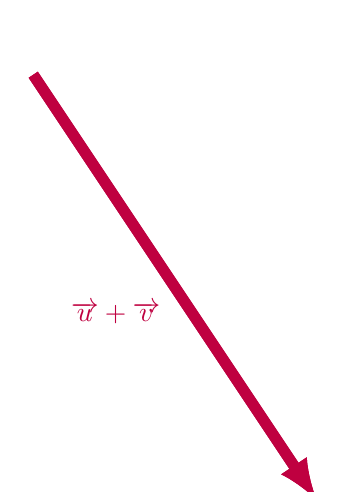
\begin{tikzpicture}[scale=0.45,every node/.style={scale=1}]
		\vectAuColor{u}{5}{19}{12}{-8}{4pt}{0.5}{above right}{blue};
		\vectAuColor{v}{17}{11}{-4}{-4}{4pt}{0.5}{above left}{cyan};
		\draw[->,>=latex,line width=4pt,purple] (5,19) -- (13,7) node[fill=white,pos=0.5,below left] {$\textcolor{purple}{\overrightarrow{u} + \overrightarrow{v}}$};
		\draw[->,>=latex,line width=4pt,purple] (5,19) -- (13,7); % On retrave le vecteur sur l'étiquette du nom
	\end{tikzpicture}
	\fbox{On notera \textcolor{purple}{\vectaffiche{u} + \vectaffiche{v}} les caractéristiques de cette nouvelle transformation}
\end{center}
	
\begin{enumerate}
	\setcounter{enumi}{1}
	\item Enchaînement 2
	\vspace{-2em}
		\begin{enumerate}
			\item Quelle est l'image du carreau \zellige{38} par la translation de vecteur \vectaffiche{s}~? \textcolor{red}{C'est le carreau 40.}
			\item Quelle est l'image de cette image par la translation de vecteur~\vectaffiche{t}~?
				 \textcolor{red}{C'est le carreau 34.}
			\item Émettre une conjecture sur \vectaffiche{s} + \vectaffiche{t}. \textcolor{red}{C'est la translation de vecteur \vectaffiche{s} suivie de la translation de vecteur \vectaffiche{t}.}
		\end{enumerate}
	\item Enchaînement 3
	\vspace{-2em}
		\begin{enumerate}
			\item Quelle est l'image du carreau \zellige{22} par la translation de vecteur \vectaffiche{v}~? \textcolor{red}{C'est le carreau 15.}
			\item Quelle est l'image de cette image par la translation de vecteur~\vectaffiche{r}~?
				 \textcolor{red}{C'est le carreau 22.}
			\item Émettre une conjecture sur \vectaffiche{v} + \vectaffiche{r}. \textcolor{red}{On revient sur le carreau de départ. \vectaffiche{v} + \vectaffiche{r} est le vecteur nul :  \vectaffiche{v} + \vectaffiche{r} $=$ \vectaffiche{0}.}
		\end{enumerate}
\end{enumerate}

\end{document}
